\subsection{Multiplication matrice vecteur creuse}
La multiplication du matrice creuse par un vecteur est une opération dont le ratio nombre d'opérations par le nombre d'octet lus est petit.
%
Dans le cas d'une matrice scalaire, ce ratio vaut environ $1/10$ en double précision.
%
Pour chaque valeur non-nulles de la matrice, il faut lire cette valeur, l'indice de la colonne et la valeur contenue dans le vecteur à l'indice de la colonne.
%
Il faut ensuite multiplier les deux valeurs ensemble et l'ajouter à un accumulateur, ce qui fait en double précision 2 opérations pour 20 octets lus.
%
Si nous utilisons trois variables primaires, chaque entrée de la matrice est un bloc 3 par 3.
%
Nous devons donc lire ce bloc (9*8 Octets), lire l'indice de colonne (4 Octets) et finalement lire 3 valeurs dans le vecteur (3*8 Octets).
%
Pour chaque valeurs du bloc nous avons 2 opérations à faire (2*9), nous avons donc un ratio de $18/100$ soit environ $1/5,5$.
%
Avec huit variables primaires, le ratio monte à environ de $1/4,5$.


Le {\em roofline model} est un modèle de performance permettant de connaître la puissance de calcul maximale pouvant être atteinte par un algorithme sur une machine.
%
Ce modèle se construit de la façon suivante, dans un premier temps nous allons mesurer la bande passante maximale de la machine.
%
Pour cela nous avons utiliser le benchmark STREAM, sur Rostand, nous obtenons une bande passante de 21~Go/s.
%
Puis, dans un second temps, nous allons calculer la capacité de calcul maximale de la machine.
%
Pour calculer cette capacité, il faut multiplier le nombre de coeur de calcul par le nombre maximal d'opérations faites dans une instruction et multiplier le tout pas la fréquence d'horloge.
%
Chaque noeud de Rostand étant composé de 12 coeurs cadencés à 2,80~GHz et de l'instruction SSE~4.2 permettant d'effectuer 4 opérations flottantes à la fois, ce qui donne 134,4~GFlops.


Une fois le roofline model construit, nous pouvons donc placer le produit matrice vecteur creux.
%
Les performances du SpMV dépend du nombre de variables primaires, nous avons donc placer sur le roofline model trois SpMV en fonction du nombre de variable primaire utilisées.
%
Ces trois points nous indique que les performances du SpMV seront limitées par la bande passante mémoire.

%   (-_-)   %
\begin{figure}[t!]
  \centering
  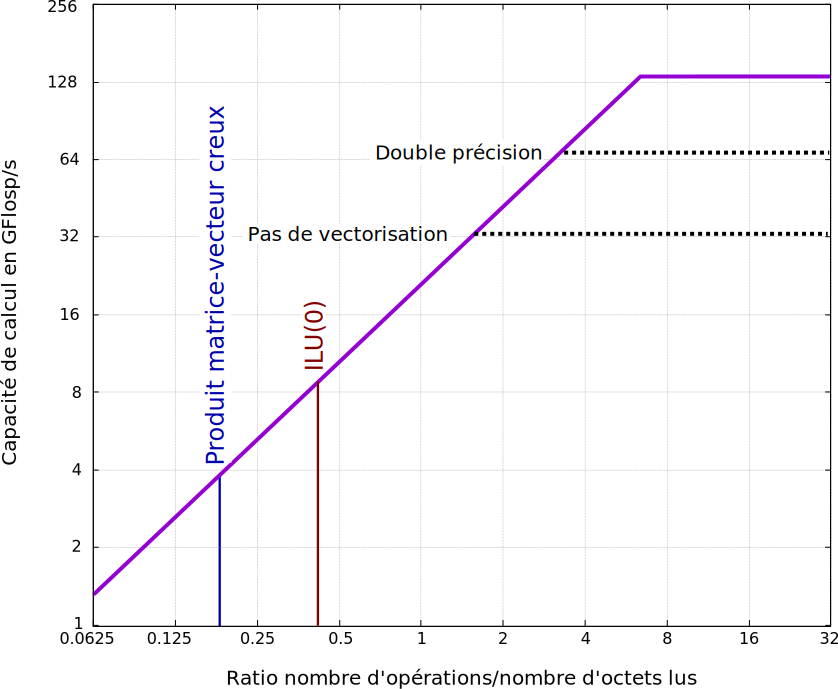
\includegraphics[width=0.8\textwidth]{roofline_rostand}
  \caption{Roofline model de Rostand. avec les différents produit matrice vecteur creux.}
  \label{fig:roofline_rostand}
\end{figure}


% -------------------------------
\subsubsection{Mémoire distribuée}
Le produit matrice vecteur creux, que j'abrégerai SpMV pour le reste des résultats, est un algorithme qui se parallélise très bien en mémoire partagée.
%
Nous pouvons donc estimer que la performance atteinte en mémoire distribuée est une borne maximale à atteindre en mémoire partagée.
%
En effet, de par sa nature distribuée, les pénalités mémoires NUMA sont minimales.
%
Le roofline model prédit un algorithme limité en performance par la bande passante mémoire.
%
Or, cette bande passante mémoire est partagée entre les coeurs d'un même banc NUMA.
%
L'accélération obtenue sera donc limité par la bande passante mémoire.
%
Sur la machine rostand, la bande passante mémoire limite grandement cette accélération (fig.~\ref{fig:res_spmv_mpi_rostand}).
%
Avec un cas à 8 variables primaires, nous obtenons une accélération maximal de 3,8.
%
La capacité de calcul mesuré avec 12 coeurs est de 4,96~GFlops, cela correspond à la prédiction du roofline model.


%   (-_-)   %
\begin{figure}[t!]
  \centering
  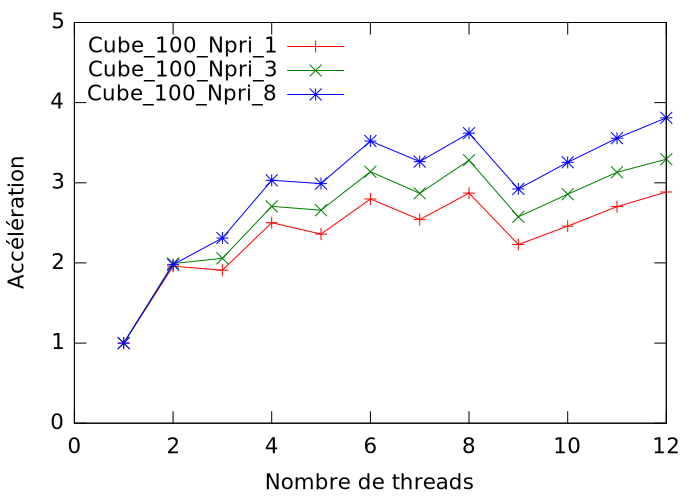
\includegraphics[width=0.7\textwidth]{res_spmv_mpi}
  \caption{Accélération du produit matrice vecteur creux sur Rostand en mémoire distribuée.}
  \label{fig:res_spmv_mpi_rostand}
\end{figure}



Sur Manumanu, nous avons beaucoup plus de banc NUMA, ce qui signifie que nous aurons plus de bande passante mémoire à notre disposition.
%
Nous pouvons donc espérer avoir de meilleurs résultats que sur Rostand.
%
Il faut aussi prendre en compte une bande passante mémoire plus élevée sur les banc NUMA de Manumanu que sur ceux de Rostand.
%
Les processus MPI sont alloués en mode compact, c'est à dire qu'ils sont distribués de façon à utiliser un minimum de noeuds NUMA.
%
Sur 1 banc NUMA, nous avons une accélération de 5 avec 8 variables primaires (fig~\ref{fig:res_spmv_mpi_manu}).
%
Cette accélération monte à 110 avec l'utilisation des 20 bancs NUMA et des 160 coeurs.


%   (-_-)   %
\begin{figure}[t!]
  \centering
  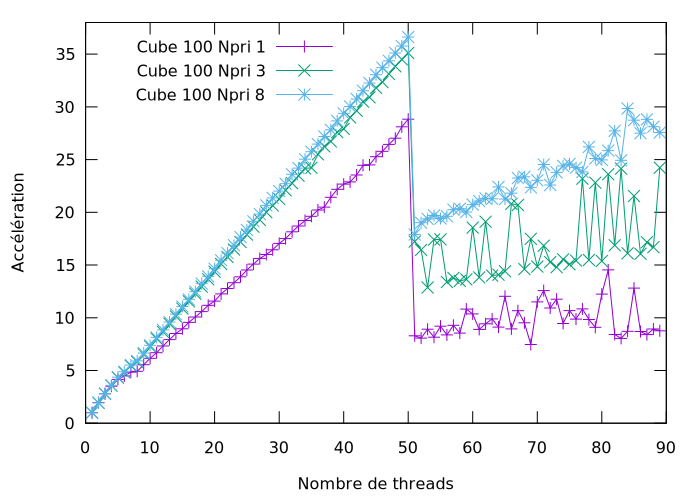
\includegraphics[width=0.7\textwidth]{res_spmv_mpi_manu}
  \caption{Accélération du produit matrice vecteur creux sur Manumanu en mémoire distribuée.}
  \label{fig:res_spmv_mpi_manumanu}
\end{figure}

% -------------------------------
\subsection{First touch}
Les résultats de la factorisation et de la résolution triangulaire avec une allocation first touch sont exposés dans le chapitre précèdent.
%
Les résultats ne sont pas aussi bons que ceux que nous pourrions obtenir avec une meilleure gestion de la mémoire.
%% TODO résultat manumanu


Le produit matrice vecteur creux ne passe pas à l'échelle.
%
Nous obtenons difficilement une accélération de 2,5 sur 12 coeurs en ayant 8 variables primaires (Fig.~\ref{fig:res_spmv_omp_rostand}).
%
Cette accélération descend à 1,9 en ayant 1 variable primaire, toujours sur 12 coeurs de calcul.
%
L'utilisation d'un paradigme en mémoire distribuée ne change pas le calcul mais garanti un placement mémoire optimal.
%
Les résultats sur le produit matrice vecteur sont bien meilleur qu'en mémoire partagée, nous atteignons une accélération de 3,8.
%
Cette différence est en grande partie dû aux effets NUMA, comme le montre la suite des expériences.


%   (-_-)   %
\begin{figure}[t!]
  \centering
  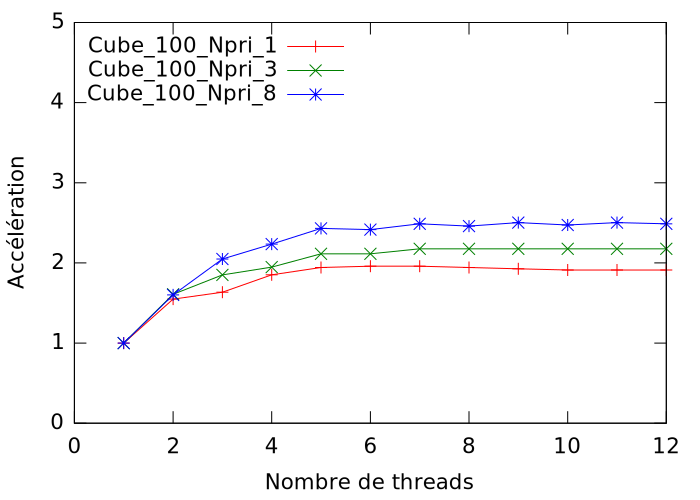
\includegraphics[width=0.7\textwidth]{res_spmv_omp}
  \caption{Accélération du produit matrice vecteur creux sur Rostand en mémoire partagée.}
  \label{fig:res_spmv_omp_rostand}
\end{figure}

%   (-_-)   %
\begin{figure}[t!]
  \centering
  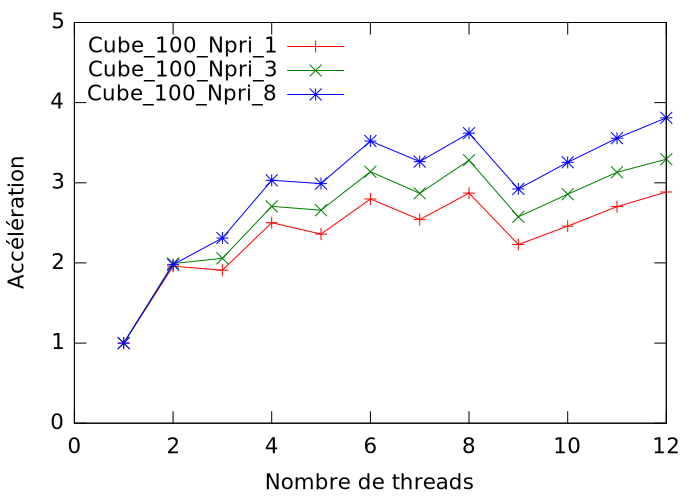
\includegraphics[width=0.7\textwidth]{res_spmv_mpi}
  \caption{Accélération du produit matrice vecteur creux sur Rostand en mémoire distribuée.}
  \label{fig:res_spmv_mpi_rostand}
\end{figure}

% -------------------------------
